% MIT License

% Copyright (c) 2019-2020 Simon Crase

% Permission is hereby granted, free of charge, to any person obtaining a copy
% of this software and associated documentation files (the "Software"), to deal
% in the Software without restriction, including without limitation the rights
% to use, copy, modify, merge, publish, distribute, sublicense, and/or sell
% copies of the Software, and to permit persons to whom the Software is
% furnished to do so, subject to the following conditions:

% The above copyright notice and this permission notice shall be included in all
% copies or substantial portions of the Software.

% THE SOFTWARE IS PROVIDED "AS IS", WITHOUT WARRANTY OF ANY KIND, EXPRESS OR
% IMPLIED, INCLUDING BUT NOT LIMITED TO THE WARRANTIES OF MERCHANTABILITY,
% FITNESS FOR A PARTICULAR PURPOSE AND NONINFRINGEMENT. IN NO EVENT SHALL THE
% AUTHORS OR COPYRIGHT HOLDERS BE LIABLE FOR ANY CLAIM, DAMAGES OR OTHER
% LIABILITY, WHETHER IN AN ACTION OF CONTRACT, TORT OR OTHERWISE, ARISING FROM,
% OUT OF OR IN CONNECTION WITH THE SOFTWARE OR THE USE OR OTHER DEALINGS IN THE
% SOFTWARE.

\documentclass[]{article}
\usepackage{caption,subcaption,graphicx,float,url,amsmath,amssymb,tocloft,cancel}
\usepackage[hidelinks]{hyperref}
\usepackage[toc,acronym,nonumberlist]{glossaries}
\usepackage{titling}
\setacronymstyle{long-short}
\usepackage{glossaries-extra}
\graphicspath{{figs/}} 
\setlength{\cftsubsecindent}{0em}
\setlength{\cftsecnumwidth}{3em}
\setlength{\cftsubsecnumwidth}{3em}
% I snarfed the next line from Stack exchange
% https://tex.stackexchange.com/questions
%    /42726/align-but-show-one-equation-number-at-the-end
% It allows me to suppress equation numbers with align*,
% then selectively add equation numbers
% for lines that I want to reference slsewhere
\newcommand\numberthis{\addtocounter{equation}{1}\tag{\theequation}}
% Add logo at start of document


%opening
\title{
	Notes from \\
	Computation in Complex Systems
}
\author{Simon Crase (compiler)\\simon@greenweaves.nz}

\makeglossaries


%\loadglsentries{glossary-entries}

\renewcommand{\glstextformat}[1]{\textbf{\em #1}}

\begin{document}

\maketitle

\begin{abstract}
   These are my notes from Computation in Complex Systems\
   The content and images contained herein are the intellectual property of the Santa Fe Institute, with the exception of any errors in transcription, which are my own.
   These notes are distributed in the hope that they will be useful,
   but without any warranty, and without even the implied warranty of
   merchantability or fitness for a particular purpose. All feedback is welcome,
   but I don't necessarily undertake to do anything with it.\\
   \LaTeX source for this week's lectures can be found at\\
   \url{https://github.com/weka511/complexity/tree/master/origins}.
\end{abstract}

\setcounter{tocdepth}{2}
\tableofcontents

\listoffigures



\newglossaryentry{gls:O}{
	name={O},
	description={$f(n)=O(n^3)$ means: when $n$ is large $f(n)$ scales as $n^3$ or less. Formally:
	\begin{align*}
		f(n) =& O(g(n))\\
		\equiv&	\;\; \exists C, n_0 \text{ such that}\\
		 \forall n>n_0, f(n) \le& Cg(n)
	\end{align*}}}

\newglossaryentry{gls:Omega}{
	name={$\Omega$},
	description={$f$ grows at least as fast as $g$: $g=O(f)$ : $f/g \cancel{\rightarrow} 0 \text{ as } n\rightarrow \infty$}}

\newglossaryentry{gls:Theta}{
	name={$\Theta$},
	description={$f$ and $g$ grow the same way: $g=O(f)$ and $f=O(g)$ or $f/g \rightarrow C>0\text{ as } n\rightarrow \infty$}}

\newglossaryentry{gls:o}{
	name={o},
	description={$f$ grows more slowly than $g$: $f/g \rightarrow 0 \text{ as } n\rightarrow \infty$}}

\section{Easy \& Hard}

\cite[Chapters 1,2,4]{moore2011nature}

For theorists, polynomial vs. exponential is the mark of insight: we have found some structure in the problem that we can use.

\subsection{Two Kinds of Paths}

\subsection{Polynomials vs. Exponentials}

\subsection{Divide and Conquer}

\subsection{Big O and All that}

\subsection{When the details don't matter}

\section{Algorithms and Landscapes}
\cite[Chapter 2]{moore2011nature}

\subsection{Divide and Conquer Redux}

\subsection{Dynamic Programming}

\begin{align*}
	d(s,t)=& \min(d(s^\prime,t)+1, d(s,t^\prime)+1,d(s^\prime,t^\prime) + \delta(s_1,t_1)) \text{ , where}\\
	d(s,t)=& \text{ number of changes to convert $s$ to $d$}\\
	s^\prime=& \text{ string $s$ with 1st character, $s_1$ removed}\\
	t^\prime=& \text{ string $t$ with 1st character, $t_1$ removed}
\end{align*}

There are only $n^2$ sub-problems: polynomial time.

\subsection{Greedy Algorithms}

\begin{figure}[H]
	\caption{Minimum Spanning Tree}
	\begin{subfigure}[t]{0.45\textwidth}
		\caption{e.g. power lines}
		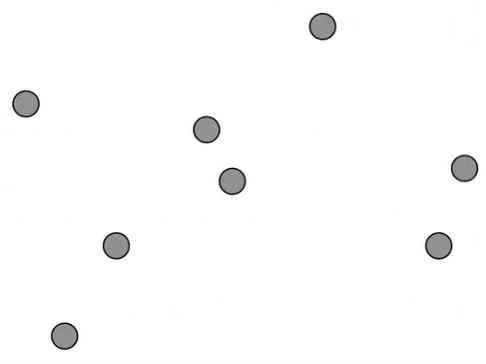
\includegraphics[width=\textwidth]{mst1}
	\end{subfigure}
	\;\;\;
	\begin{subfigure}[t]{0.45\textwidth}
		\caption{Start by adding the shortest edge}
		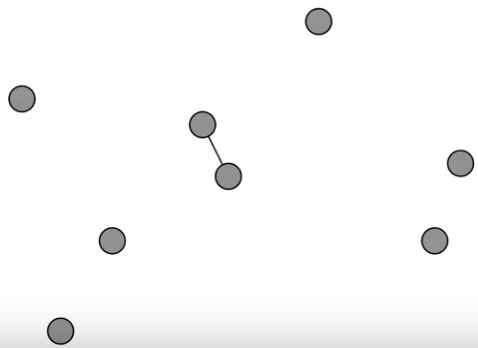
\includegraphics[width=\textwidth]{mst2}
	\end{subfigure}
	\begin{subfigure}[b]{0.45\textwidth}
		\caption{At each step, add the shortest edge that doesn't complete a cycle}
		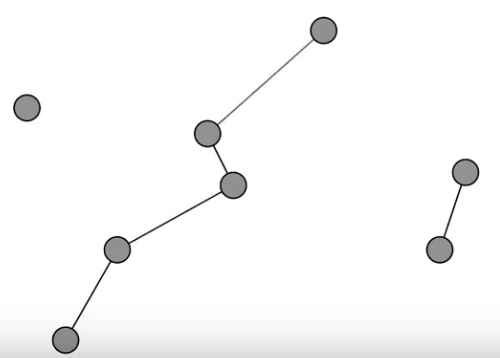
\includegraphics[width=\textwidth]{mst3}
	\end{subfigure}
	\;\;\;
	\begin{subfigure}[b]{0.45\textwidth}
		\caption{The complete tree}\label{fig:mst4}
		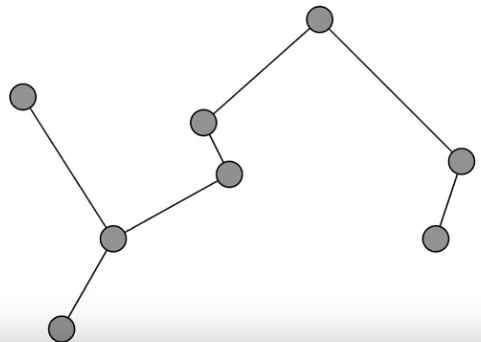
\includegraphics[width=\textwidth]{mst4}
	\end{subfigure}
\end{figure}

Clearly Figure \ref{fig:mst4} is \emph{a} spanning tree, but how do we know it is minimal?

\begin{figure}[H]
	\caption{How do we know Figure \ref{fig:mst4} is minimal?}
	\begin{subfigure}[b]{0.30\textwidth}
		\caption{Let $e$ be the shortest edge that doesn't complete a cycle, and suppose that the minimum spanning tree $T$ doesn't contain $e$}
		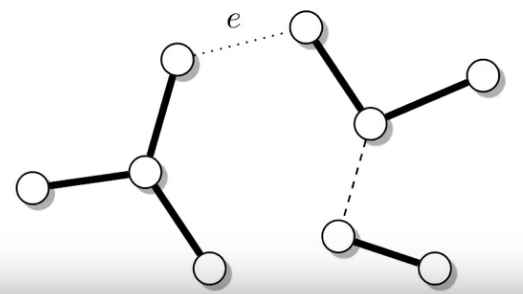
\includegraphics[width=\textwidth]{mst5}
	\end{subfigure}
	\;\;\;
	\begin{subfigure}[b]{0.30\textwidth}
		\caption{Then there must be some other path from one end of $e$ to another that goes through a longer edge $e^\prime$.}
		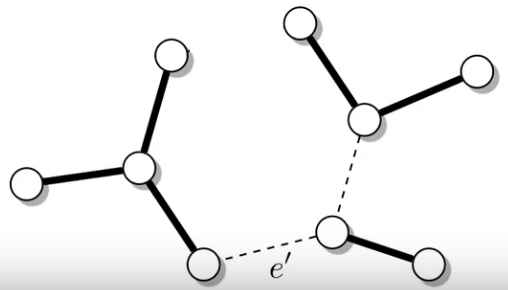
\includegraphics[width=\textwidth]{mst6}
	\end{subfigure}
	\;\;\;
	\begin{subfigure}[b]{0.30\textwidth}
		\caption{But then we could reduce the total length by deleting $e^\prime$ and adding $e$--a contradiction.}
		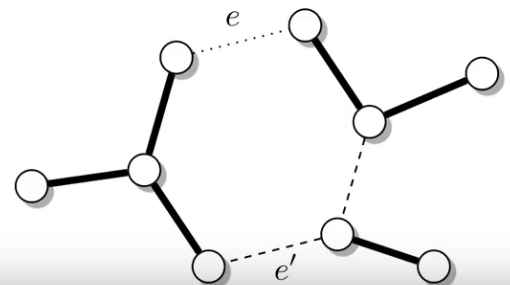
\includegraphics[width=\textwidth]{mst7}
	\end{subfigure}
\end{figure}

Greed isn't always good, or even very often good--Figures \ref{fig:greedy:tsp} and \ref{fig:lessgreedy:tsp}.
\begin{figure}[H]
	\caption{Travelling Salesman Problem}
	\begin{subfigure}[t]{0.45\textwidth}
		\caption{Greedy solution to Travelling Salesman Problem}\label{fig:greedy:tsp}
		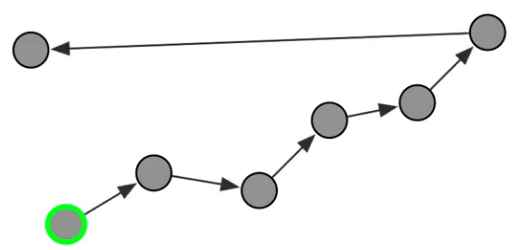
\includegraphics[width=\textwidth]{tsp1}
	\end{subfigure}
	\;\;\;
	\begin{subfigure}[t]{0.45\textwidth}
		\caption{A less Greedy solution is somewhat better}\label{fig:lessgreedy:tsp}
		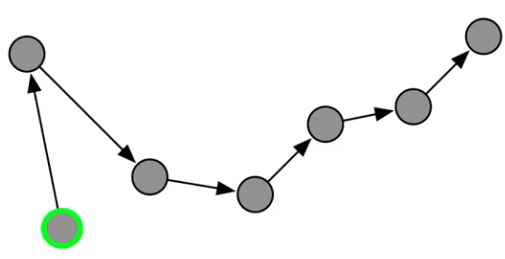
\includegraphics[width=\textwidth]{tsp2}
	\end{subfigure}
\end{figure}

\subsection{Landscapes}

\subsubsection{Greedy Algorithms and the Fitness Landscape}

\begin{figure}[H]
	\caption{Greedy Algorithms and the Fitness Landscape}
	\begin{subfigure}[t]{0.4\textwidth}
		\caption{A greedy algorithm works well if the Fitness Landscape looks like Fuji-San}
		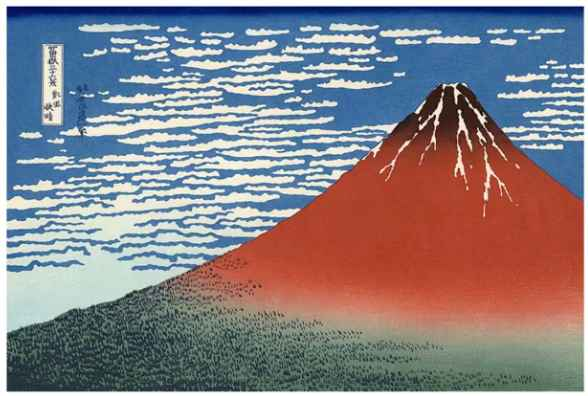
\includegraphics[width=\textwidth]{fujisan}
	\end{subfigure}
	\;\;\;
	\begin{subfigure}[t]{0.55\textwidth}
		\caption{A Greedy solution doesn't work well if there are many local optima where we can get stuck: it cannot cross a valley to get to a higher peak.}
		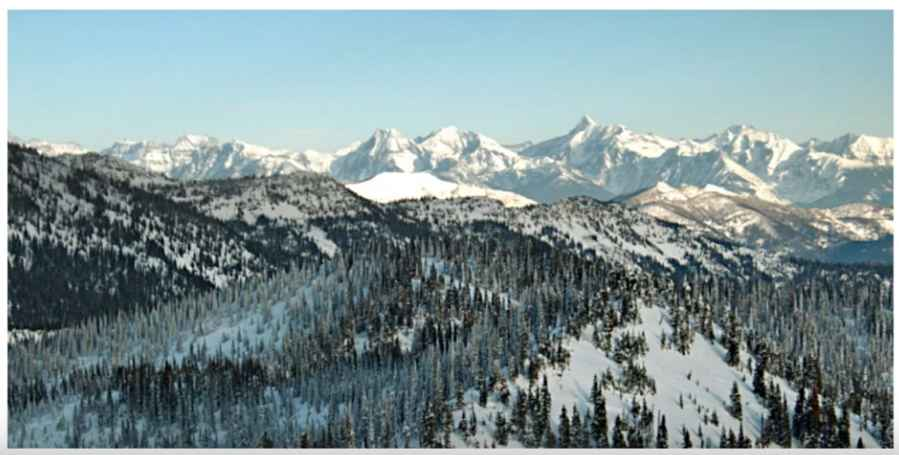
\includegraphics[width=\textwidth]{rockies}
	\end{subfigure}
\end{figure}

\subsubsection{Reorganizing the Landscape}

What defines the neighbourhood? When is one solution close to another?

\begin{figure}[H]
	\caption{Maxflow: take a network such as \ref{fig:maxflow1} and determine the maximum flow from $s$ to $t$. We can see that we can eliminate local optima by allowing a new kind of move. By expanding our idea of what kins of solutions are neighbours we reorganize the landscape!}
	\begin{subfigure}[t]{0.4\textwidth}
		\caption{Each edge has a capacity}\label{fig:maxflow1}
		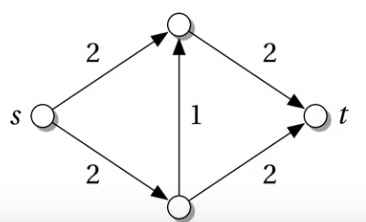
\includegraphics[width=\textwidth]{maxflow1}
	\end{subfigure}
	\;\;\;
	\begin{subfigure}[t]{0.55\textwidth}
		\caption{Greedy: push more flow along a channel with excess capacity. But we can get stuck at a local optimum. Here we have three units flowing--we are at a local optimum.}\label{fig:maxflow2}
		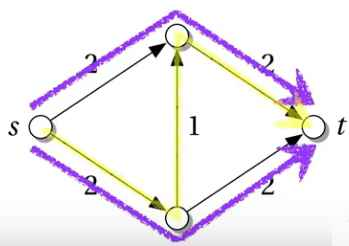
\includegraphics[width=\textwidth]{maxflow2}
	\end{subfigure}
	\;\;\;
	\begin{subfigure}[t]{0.45\textwidth}
		\caption{We should have done this instead}\label{fig:maxflow3}
		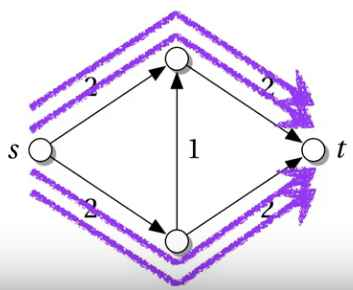
\includegraphics[width=\textwidth]{maxflow3}
	\end{subfigure}
	\;\;\;
	\begin{subfigure}[t]{0.45\textwidth}
		\caption{Allow reverse edges to cancel previous flow: now if we add to Figure \ref{fig:maxflow2} we get the optimum--Figure \ref{fig:maxflow3}. If we allow this type of move we can never get stuck: there are no local optima.}
		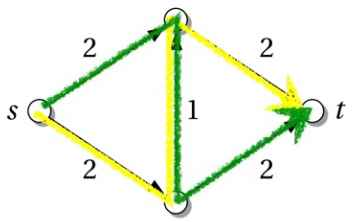
\includegraphics[width=\textwidth]{maxflow4}
	\end{subfigure}
\end{figure}

This won't always work. Some problems are inherently bumpy.

\subsection{Reductions and Translations}

\begin{figure}[H]
	\caption{Shortest Path}
	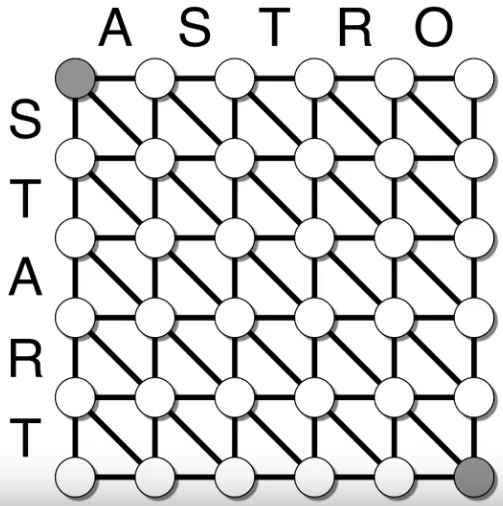
\includegraphics[width=0.8\textwidth]{sp1}
\end{figure}

\subsection{Lessons So Far}

\subsection{The Best of All Possible Algorithms}

\subsection{Complexity Wrap-Up}

\begin{itemize}
	\item \emph{Systems} aren't simple or complex; questions about them are.
	\item Intrinsic complexity of a problem: the running time, or memory, or other resource, of the \emph{best possible algorithm}; an objective mathematical fact.
	\item Upper bounds are easy: just give an algorithm.
	\item Lower bounds are hard.
	\item Lower bounds show that one problem is at least as easy (or hard) as another. 
\end{itemize}

\section{P versus NP}
\cite[Chapters 4-6]{moore2011nature}, \cite{sep-computability}

\subsection{Finding versus Checking}

\subsection{Circuits and Formulae}

\subsection{More NP-complete Problems}

\subsection{P versus NP Problem}

\subsection{Existence and Nonexistence }

\subsection{Above and Beyond}

\section{Worst-case, Natural, and Random}
\cite[Chapters 5,10]{moore2011nature}
\section{Computation Everywhere}
\cite[Chapter 7]{moore2011nature}
% end of text 

% glossary
\glsaddall
\printglossaries

% bibliography go here
 
\bibliographystyle{unsrt}
\addcontentsline{toc}{section}{Bibliography}
\bibliography{computations}

\end{document}
